\input ../SlidePreamble
\input ../preamble

\begin{document}

{\Huge
  \centerline{\bf TTIC 31230,  Fundamentals of Deep Learning}
  \vfill
  \centerline{David McAllester, Autumn 2023}
  \vfill
\centerline{Some Information Theory}

\slide{Why Information Theory?}

The fundamental equation of deep learning involves cross-entropy.

\vfill
Cross-entropy is an information-theoretic concept.

\vfill
Information theory arises in many places and many forms in deep learning.

\slide{Entropy of a Distribution}

The entropy of a distribution $P$ is defined by

\vfill
$${\color{red} H(P) = E_{y \sim P} \left[ \;- \ln P(y)\right]}\;\;\mbox{in units of ``nats''}$$

\vfill
$${\color{red} H_2(P) = E_{y \sim P}\left[ \;- \log_2 P(y)\right]}\; \mbox{in units of bits}$$

\slide{Why Bits?}

Why is $-\log_2\;P(y)$ a number of bits?

\vfill
Example: Let $P$ be a uniform distribution on 256 values.

\vfill
$$E_{y \sim P}\;\left[\;-\log_2 P(y)\right] = - \log_2 \frac{1}{256} = \log_2 256 = 8\;\mathrm{bits} = 1\;\mathrm{byte}$$

\vfill
\centerline{\color{red} 1 nat = $\frac{1}{\ln 2}$ bits $\approx$ 1.44 bits}

\slide{Shannon's Source Coding Theorem}

Why is $-\log_2\;P(y)$ a number of bits?

\vfill
A prefix-free code for ${\cal Y}$ assigns a bit string $c(y)$ to each $y \in {\cal Y}$ such that no code string is prefix of any other code string.

\vfill
For a probability distribution $P$ on ${\cal Y}$ we consider the average code length $E_{y \sim P}\;\left[ \;|c(y)|\right]$.

\vfill
Theorem: For any $c$ we have {\color{red} $E_{y \sim P}\;|c(y)|  \geq H_2(P)$}.

\vfill
Theorem: There exists $c$ with {\color{red} $E_{y \sim P} \;|c(y)| \leq H_2(P) +1$}.

\slide{Cross Entropy}

Let $P$ and $Q$ be two distribution on the same set.

{\color{red} $$H(P,Q) = E_{y \sim P}\;\left[ \;-\ln \;Q(y)\right]$$}

{\color{red} $$\Phi^* = \argmin_\Phi \;H(\pop,P_\Phi)$$}

\vfill
{\color{red} $H(P,Q)$} can be interpreted as the number of bits used to code draws from $P$ when using an optimal code for $Q$.

\vfill We will show
$$H(P,Q) \geq H(P)$$

\slide{KL Divergence}

Let $P$ and $Q$ be two distribution on the same set.

\vfill
\centerline{
  $\begin{array}{lrcl}
\mathrm{Entropy}: & {\color{red} H(P)} & = & {\color{red} E_{y \sim P}\;\left[-\ln\;P(y)\right]} \\
\\
\mathrm{Cross Entropy:} & {\color{red} H(P,Q)} & = & {\color{red} E_{y \sim P}\;\left[-\ln\;Q(y)\right]} \\
\\
\mathrm{KL\; Divergence:} & {\color{red} KL(P,Q)} & = & {\color{red} H(P,Q) - H(P)} \\
\\
& & = & {\color{red} E_{y \sim P}\;\;\; - \ln\;\frac{Q(y)}{P(y)}}
\end{array}$}

\vfill
We will show $KL(P,Q) \geq 0$ which implies $H(P,Q) \geq H(P)$.

\slideplain{Proving $KL(P,Q) \geq 0$: Jensen's Inequality}

\centerline{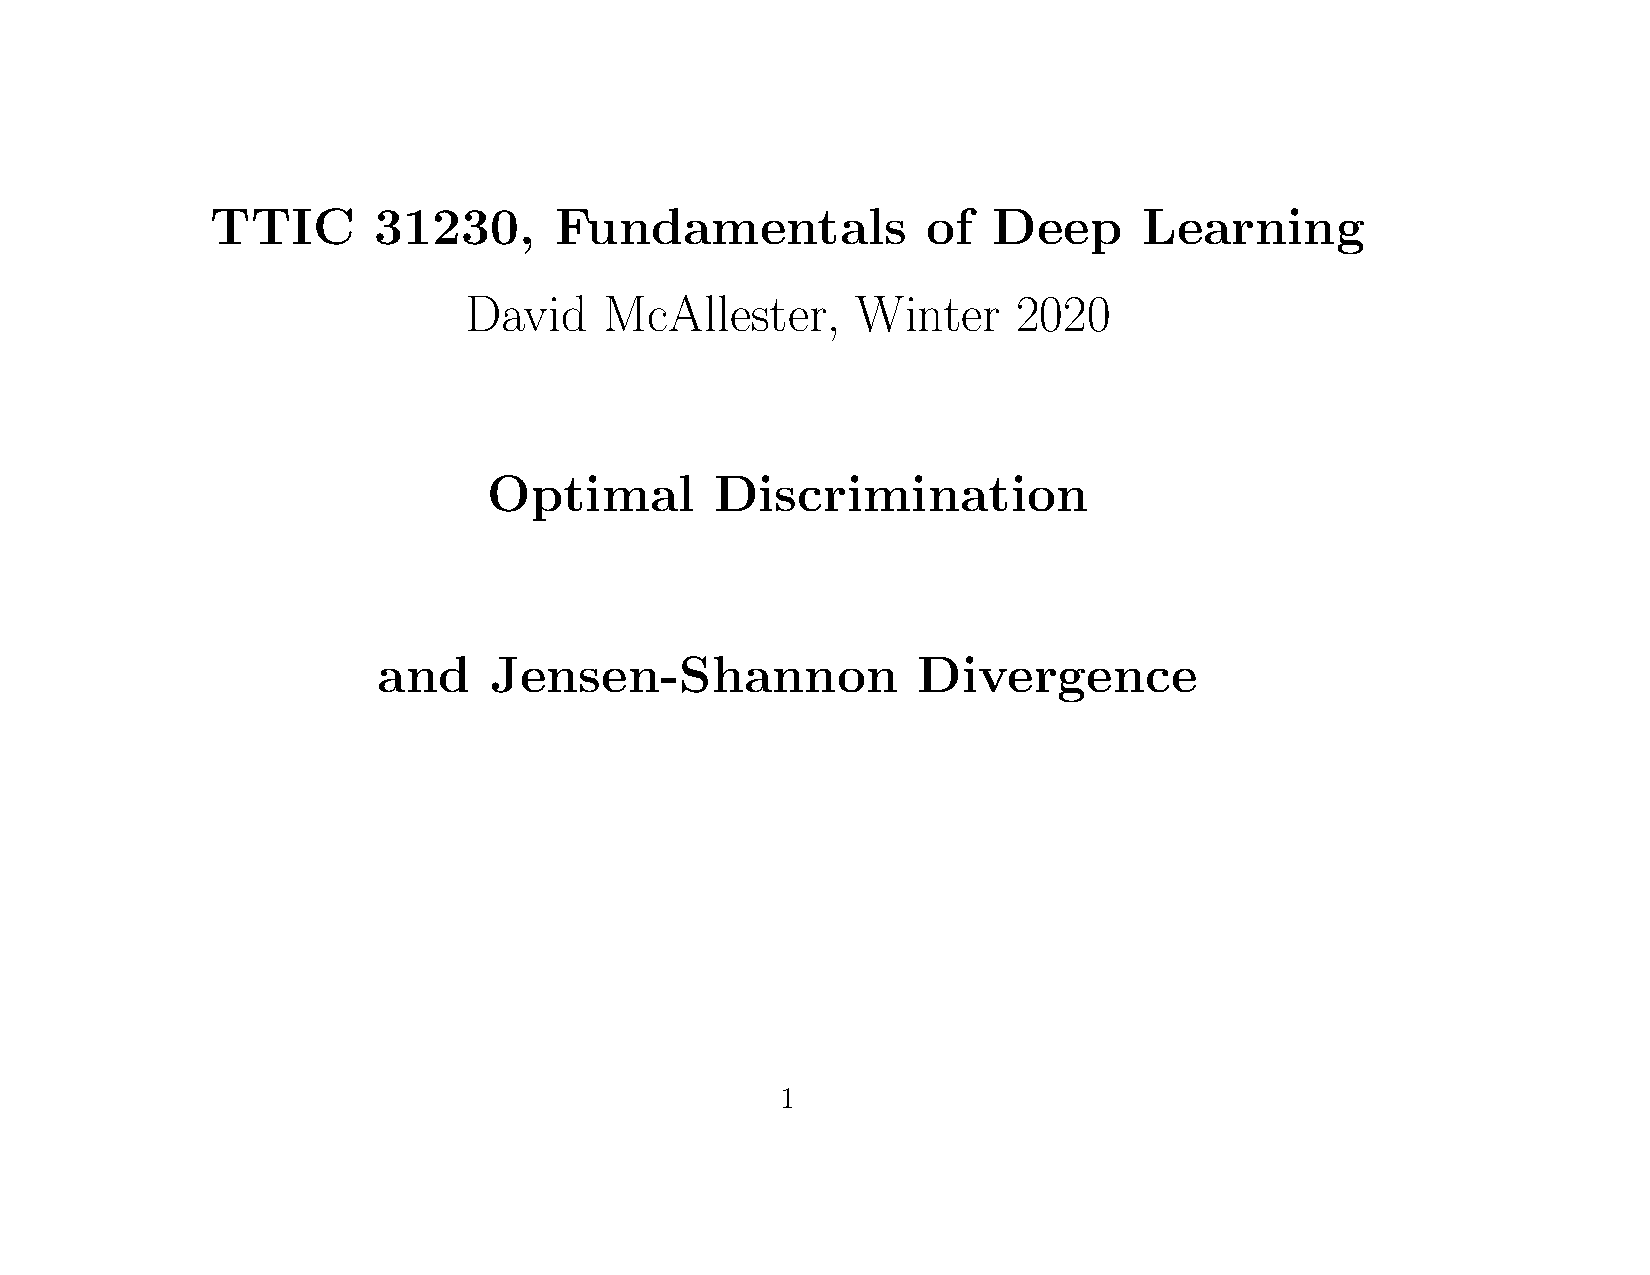
\includegraphics[height = 3.0in]{\images/Jensen}}

\vfill
For $f$ convex (upward curving) we have

\vfill
$$E[f(x)] \geq f(E[x])$$

\slide{Proving $KL(P,Q) \geq 0$}

\begin{eqnarray*}
  KL(P,Q) & = & \expectsub{y \sim P}{\left[- \ln \frac{Q(y)}{P(y)}\right]} \\
  \\
  & \geq & - \ln \expectsub{y\sim P}{\frac{Q(y)}{P(y)}} \\
  \\
  & = & - \ln \sum_y\; P(y) \frac{Q(y)}{P(y)}  \\
  \\
  & = & - \ln \sum_y Q(y) \\
  \\
  & = & 0
\end{eqnarray*}



\slide{Asymmetry of Cross Entropy}
Consider 


$$\Phi^* = \argmin_\Phi \;H(\pop,Q_\Phi)\;\;\;\;\;(1)$$

\vfill
$$\Phi^* = \argmin_\Phi \;H(Q_\Phi,\pop)\;\;\;\;\;(2)$$

\vfill
We cannot use (2) because we cannot calculate $\pop(y)$.

\vfill
For a synthetic population where $\pop(y)$ is computable (2) produces mode collapse --- $Q_\Phi$ is concentrated on the most likely value of $\pop$.

\slide{Asymmetry of KL Divergence}
Consider 


\begin{eqnarray*}
  \Phi^* & = & \argmin_\Phi \;KL(\pop,Q_\Phi) \\
  & = & \argmin_\Phi\; H(\pop,Q_\Phi)\;\;\;\;\;\;\;\;\;\;\;\;\;\;\;\;\;\;(1) \\
  \\
  \Phi^* & = & \argmin_\Phi \;KL(Q_\Phi,\pop) \\
  & = & \argmin_\Phi H(Q_\Phi,\pop) - H(Q_\Phi)\;\;\;(2)
  \end{eqnarray*}

\vfill
For a synthetic population where $\pop(y)$ is computable but $P_\Phi$ cannot perfectly model $\pop$, (2) produces mode collapse.

\slide{Conditional Entropy and Mutual Information}

Assume a joint distribution $Q$  on $x$ and $y$.

\vfill
conditional entropy:
$$H(y|x) = E_{(x,y)\sim Q}\;-\ln P(y|x)$$

\vfill
mutual information:
$$I(x,y) = H(y) - H(y|x)$$

\vfill
Suppose you dont't know anything about $x$ and $y$. The mutual information $I(x,y)$ is the expectation over a draw of $x$ of
the number of bits you learn about $y$.

\slide{Summary}
      
\centerline{
  $\begin{array}{lrcl}
\mathrm{Entropy}: & {\color{red} H(P)} & = & {\color{red} E_{y \sim P}\;\left[-\ln\;P(y)\right]} \\
\\
\mathrm{Cross Entropy:} & {\color{red} H(P,Q)} & = & {\color{red} E_{y \sim P}\;\left[-\ln\;Q(y)\right]} \\
\\
\mathrm{KL\; Divergence:} & {\color{red} KL(P,Q)} & = & {\color{red} H(P,Q) - H(P)} \\
\\
\mathrm{Mutual\; Information:} & {\color{red} I(x,y)} & = & {\color{red} H(y) - H(y|x)}
\end{array}$}

\vfill
\centerline{{\color{red} $H(P,Q) \geq H(P),\;\;\;KL(P,Q) \geq 0,\;\;\;\argmin_Q\;H(P,Q) = P$}}

\slide{END}

\end{document}
